\documentclass[12pt]{article}
\usepackage[T1]{fontenc}
\usepackage{lmodern,amsmath,amssymb,amsthm,graphicx,mathrsfs}
\usepackage[numbers,sort&compress]{natbib}
\usepackage[margin=1in]{geometry}
\usepackage[colorlinks=true,linkcolor=blue,citecolor=blue,urlcolor=blue]{hyperref}
\usepackage{doi}
\newtheorem{proposition}{Proposition}
\newcommand{\R}{\mathbb R}
\begin{document}
\title{Can the Journey Continue?\\
The Boundaries of Alcubierre Spacetimes}
\author{Sergei Slobodov\\
Independent researcher\\
\href{mailto:sergei@slobodov.com}{\texttt{sergei@slobodov.com}}}
\date{}
\maketitle

\begin{abstract}
A freely falling traveler can reach the front of an Alcubierre warp
bubble in finite time on their own clock, while time at the bubble's
center grows without bound. Does the journey end there? For the steadily
moving bubbles studied here, we show that a spherical wall permits no
smooth continuation of spacetime. We construct a bubble with a flat cap
through which the traveler can cross into a new region of spacetime.
We give an exact criterion for when the full four-dimensional spacetime
can be extended.
\end{abstract}

\section{Introduction}

A freely falling traveler in an Alcubierre bubble \cite{Alcubierre1994}
can approach its front wall in finite proper time, while the time shown
by a clock at the bubble's center tends to infinity. We ask whether the
traveler's path can continue in an extension, a larger spacetime that
contains the entire original spacetime and preserves its metric.

We fix the two transverse coordinates at their values on the bubble's
axis, leaving a two-dimensional slice with coordinates for time and
position along the axis. The metric on this slice admits a smooth
continuation \cite{FinazziLiberatiBarcelo2009}.
For the four-dimensional stationary bubbles specified in
Section~\ref{extensions}, we show that a spherical wall rules out any
extension with a twice continuously differentiable (\(C^2\)) metric.
We construct a compact bubble with the same metric on this slice as a
spherical bubble. The traveler can cross through its flat cap into a
smooth extension.

On this two-dimensional slice, the front of the bubble behaves like a
white-hole horizon \cite[Sec.~2 and Fig.~1]{BarceloEtAl2022}. Light sent
forward from inside the bubble approaches the front only as the time on
the central clock tends to infinity. On an open planar patch of the wall
perpendicular to the direction of travel,
neighboring forward-directed light rays stay at fixed positions in the
bubble's coordinates. Their paths generate a Killing horizon in the
full spacetime.
The surface gravity of this horizon is the slope of the forward coordinate
speed of light as one moves straight through the wall
\cite[cf. Eq.~(13)]{FinazziLiberatiBarcelo2009}. The metric on the slice
gives this slope where the axis meets the wall.

Our main result is a criterion for extending the full four-dimensional
spacetime. A bubble with a regular wall admits a \(C^2\) extension
exactly when the wall contains an open planar patch perpendicular to
travel with constant, nonzero surface gravity. The planar patch is
necessary even for an irregular wall. For a globally real-analytic
profile, the wall value on an open planar patch would persist across the
entire transverse plane, contrary to the exterior limit. Such profiles
are therefore \(C^2\)-inextendible.

R\'acz and Wald showed how to extend a neighborhood of a Killing horizon
with constant, nonzero surface gravity \cite{RaczWald1992,RaczWald1996}.
For a patch satisfying our criterion, we show how to attach that local
continuation to the whole original spacetime. Gonz\'alez-D\'iaz continued
the axial metric and proposed a four-dimensional lift for a spherical
bubble \cite[Sec.~II, Eqs.~(2.10)--(2.11)]{GonzalezDiaz2000}. Our criterion
rules out a \(C^2\) extension of the full spacetime for his analytic
spherical profile.

Section~\ref{extensions} specifies the class of bubbles and derives the
corollaries. Section~\ref{compact} constructs the capped bubble and the
inextendible examples. Section~\ref{discussion} discusses nonuniqueness
and stability.

\section{Extensions of stationary bubbles}
\label{extensions}

For the stationary metrics below, we prove that a bubble with a regular
wall admits an extension exactly when the wall
contains an open planar patch perpendicular to travel, with constant
nonzero surface gravity. This excludes spherical walls.
We explain why any extension requires this patch and how the patch permits
continuation.
Appendix~\ref{app:criterion} gives the full proof.

We use the Alcubierre metric in coordinates that move with the bubble
\cite[Sec.~II, Eq.~(2)]{BarceloEtAl2022}. We take a time-independent shift
along the \(x\) axis, described by \(v\).
On \(M=\R^4\), write
\begin{equation}
 g=-dt^2+[dx-v(\boldsymbol{x})dt]^2+dy^2+dz^2,
 \qquad \boldsymbol{x}=(x,y,z),\quad r=|\boldsymbol{x}|.
 \label{metric}
\end{equation}
Assume \(v\) is smooth, \(v\leq0\), and, for some \(v_s>1\), either
\(v=-v_s\) outside a compact set or
\begin{equation}
 |v+v_s|+|\nabla v|\leq Ce^{-\sigma r}\qquad(r\geq R_0),
 \quad C,\sigma,R_0>0.
 \label{tail}
\end{equation}
These hypotheses bound \(v,\nabla v\) and make
\(\Sigma=\{v=-1\}\) compact. An extension means a connected,
time-oriented Hausdorff Lorentzian manifold with a \(C^2\) metric
containing \((M,g)\) isometrically as a proper open subset.
No field equation or energy condition is imposed.

\begin{proposition}[Extension criterion]
\label{criterion}
If \(\nabla v\ne0\) on \(\Sigma\), then \((M,g)\) admits an extension if and only if
there are \(x_H\in\R\), a nonempty open disk \(D_0\subset\R^2_{y,z}\),
and a constant \(\alpha\ne0\) such that
\begin{equation}
 v(x_H,y,z)=-1,\qquad v_x(x_H,y,z)=\alpha
 \qquad ((y,z)\in D_0).
 \label{patch}
\end{equation}
When this condition holds, a smooth extension can be attached over every
disk \(D\) with \(\overline D\subset D_0\).
\end{proposition}

Condition~\eqref{patch} requires an open planar patch on which the
derivative \(v_x\) is constant. Time translation of the patch gives a
Killing horizon for \(\chi=\partial_t\), with
surface gravity \(\alpha\), since \(\nabla_\chi\chi=\alpha\chi\)
\cite[Eq.~(1)]{RaczWald1996}.

The exterior assumption excludes escape to spatial infinity in finite
proper time. A timelike geodesic that leaves the original spacetime must
therefore approach \(\Sigma\), with an unbounded boost relative to the
stationary frame. Curvature components in nearby transported frames must
remain bounded. These bounds imply \eqref{patch}.
Conversely, the R\'acz--Wald construction extends the metric through the
patch \cite{RaczWald1992}. The appendix checks that this local extension
can be attached to the whole original spacetime.

If \(\Sigma\) is a sphere, it contains no open transverse disk and the
spacetime is \(C^2\)-inextendible. The proof uses wall regularity only to
conclude \(\alpha\ne0\), so absence of a disk excludes extensions even
when \(\Sigma\) is irregular.
If \(v\) is globally real analytic, equality \(v=-1\) on an open transverse
disk implies equality on the entire transverse plane by the identity
theorem, contradicting the exterior limit. Such profiles are therefore
also \(C^2\)-inextendible.

\section{A compact bubble with a regular extension}
\label{compact}

We construct a compact bubble with a flat cap through which a freely
falling traveler can enter a smooth extension in finite proper time
(Fig.~\ref{comparison}). We compare it with a spherical bubble that has
the same metric on the axis. We also construct a bubble with no regular
extension whose metric and all its derivatives agree on the axis with
those of the capped bubble. These examples show why a
two-dimensional diagram and the tidal forces measured by a traveler do
not determine whether the four-dimensional spacetime extends.

\begin{figure}[!t]
 \centering
 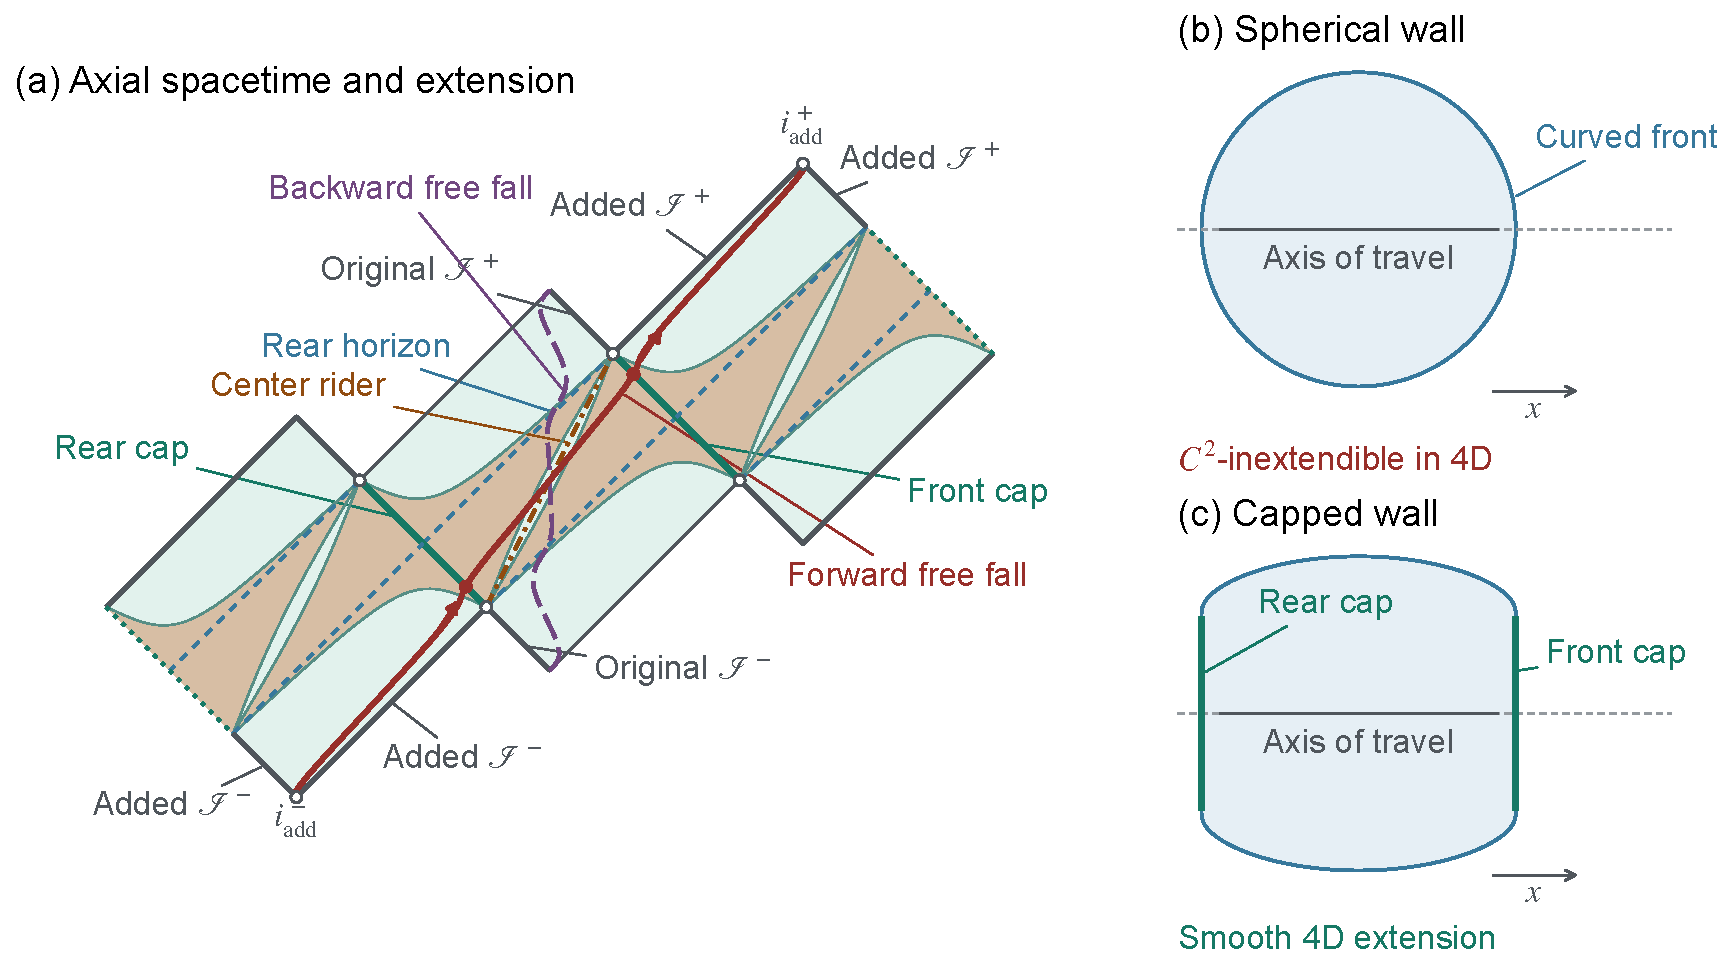
\includegraphics[width=\linewidth]{images/bubble_comparison.pdf}
 \caption{Spacetime extendibility for spherical and planar-capped bubbles.
 (a) The middle diamond is the original axial spacetime shared by both bubbles.
 The side diamonds show one smooth extension of the capped bubble. In all
 three diamonds, the exactly flat core and exteriors are light teal and the
 curved walls are darker beige. Short blue dashes mark axial horizons.
 Dotted green edges mark possible further attachments. The center rider
 (orange dash-dot) and the backward free-falling traveler (long purple dashes)
 stay in the middle diamond. The forward free-falling traveler (solid red)
 passes from \(i^-_{\mathrm{add}}\) through both caps, marked by filled dots,
 toward \(i^+_{\mathrm{add}}\).
 (b,c) Wall sections at fixed \(t\) and \(z=0\). The metrics agree on the
 axis of travel. Only the capped bubble admits a \(C^2\) extension.}
 \label{comparison}
\end{figure}

The two profiles differ only in their transverse shape:
\begin{equation}
 v_{\rm cap}=W\!\left(x^2+\psi(y^2+z^2)-1\right),\qquad
 v_{\rm sph}=W\!\left(x^2+y^2+z^2-1\right).
 \label{examples}
\end{equation}
\begin{samepage}
The function \(W\) sets the transition from the flat core to the constant
exterior. Choose it smooth and nonincreasing, with \(W(\phi)=0\) near
\(\phi=-1\), \(W(\phi)=-1-\phi/2\) near \(\phi=0\), and
\(W(\phi)=-2\) for sufficiently large \(\phi\).
Require \(W(\phi)=-1\) only at \(\phi=0\).
\par
\end{samepage}

The function \(\psi\) produces planar caps at the front and rear.
For \(0<a<1\), choose it smooth and unbounded, with \(\psi(s)=0\) for
\(s\leq a^2\), \(\psi'(s)>0\) for \(s>a^2\), and \(\psi(1)=1\).
The resulting wall is smooth, regular, and compact, with cap disks
\(x=\pm1,\rho<a\), where \(\rho^2=y^2+z^2\). On these disks
\(v_x=\mp1\), so \eqref{patch} holds.
Regularity follows from \(2x\ne0\) off the equator and \(\psi'(1)>0\)
on it. Since \(\psi(0)=0\), the capped and spherical profiles agree on
the axis. The spherical wall contains no open planar disk and admits no
regular extension.

A freely falling traveler launched from \(x=y=z=0\) along the axis with
initial momentum \(P_0>0\) follows a timelike geodesic satisfying
\(\dot x=\sqrt{P_0^2+v^2}\geq P_0\), so the traveler
reaches \(x=1\) in finite proper time. Near the cap, \(\delta=1-x\) gives
\(\dot x=E+O(\delta)\) and \(\dot t=E/\delta+O(1)\), with
\(E=\sqrt{1+P_0^2}\). Thus \(\delta e^t\to C\in(0,\infty)\).
In the regular coordinates \(U=e^{-t}\), \(V=(x-1)e^t\) of
Appendix~\ref{app:criterion}, the traveler reaches \(U=0,V=-C\) and
continues through \(U=0\).

The traveler's motion beyond either crossing depends on the metric in the
added regions. For Figure~\ref{comparison}, we continue the same shift
profile into a flat exterior in the future and use its time reverse at
the rear cap. The traveler passes from the flat past exterior to the flat
future exterior, with finite proper time between the two crossings.

We construct a bubble with no regular extension by replacing \(\psi(s)\)
in \(v_{\rm cap}\) by
\(\psi(s)+\epsilon h(s)\), where \(\epsilon>0\), \(h(s)=e^{-1/s}\) for
\(s>0\), and \(h(s)=0\) otherwise. The wall remains smooth, regular, and
compact. The new transverse profile is strictly increasing for \(s>0\),
so its wall contains no open transverse disk and the spacetime is
\(C^2\)-inextendible. All metric
derivatives still agree on the axis because \(h(y^2+z^2)\) vanishes there
to every order. The traveler follows the same coordinate trajectory in
both spacetimes. Parallel transport and all covariant derivatives of the
curvature tensor agree along this trajectory.

\begin{samepage}
\section{Discussion}
\label{discussion}

The existence of a regular extension depends on the geometry transverse
to the direction of travel. Pfenning and Ford computed tidal forces in
the Alcubierre metric \cite{PfenningFord1997}, and M\"uller and Weiskopf
studied its null and timelike geodesics \cite{MullerWeiskopf2012}. Our
examples show that two spacetimes can have the same axial diagram and
the same metric derivatives on the axis, yet differ in extendibility.
R\'acz's general extension theorem likewise imposes bounds on curvature
and its derivatives in a neighborhood of an incomplete geodesic
\cite[Sec.~6]{Racz2010}.
\par
\end{samepage}

\begin{samepage}
The capped bubble has inequivalent smooth extensions, even among maximal
extensions, when the original spacetime is held fixed. A conformal
perturbation supported on the added side can vanish to first order along
the crossing geodesic while changing the scalar curvature at a fixed
proper time. Geodesic uniqueness precludes a common extension in which
the two embeddings agree on the original spacetime. Each choice admits
a maximal continuation \cite[Thm.~1]{Clarke1976}.
\par
\end{samepage}

\begin{samepage}
The global geometry of these maximal extensions and the effect of matter
or quantum backreaction remain open questions. Barcel\'o et al. found that
a flat front traps more light rays approaching the horizon than a convex
front, increasing the scope for radiation to accumulate
\cite[Sec.~3.3]{BarceloEtAl2022}.
\par
\end{samepage}

\paragraph{Acknowledgments.}
\textit{AI disclosure.} ChatGPT/Codex (OpenAI) and Claude (Anthropic)
assisted with literature searches, drafting, and algebraic checks.
The algebraic checks were verified by symbolic computation, and the
figure was checked against the axial and transverse geometry. The
supplementary material provides the scripts for these checks. The
author takes responsibility for the results, citations, and final text.

\paragraph{Data availability.}
The verification scripts, figure-generation code, and figure output
are included in the supplementary material.

\appendix
\numberwithin{equation}{section}
\section{Proof of the extension criterion}
\label{app:criterion}

To prove Proposition~\ref{criterion}, we locate a geodesic approaching the
boundary of \(M\), use bounded curvature to derive \eqref{patch}, and
construct the extension.

\subsection{Geodesics approaching the extension boundary}

Set \((T,X)=(-t,-x)\) to turn a past extension into a future extension.
The shift becomes \(\widehat v(X,y,z)=v(-X,y,z)\).

In a \(C^2\) extension there is a timelike geodesic that leaves \(M\)
\cite[Lemma~3.2 and following paragraph]{GallowayLingSbierski2018}.
Its segment in \(M\) reaches the extension point \(q_*\) at finite
proper time \(\tau_*\), with a limiting unit tangent.

Let \(E=-p_t\), \(\Gamma=dt/d\tau>0\), and \(n=(p_x,p_y,p_z)/\Gamma\),
where \(p_i\) are the covariant momenta. Use primes for \(d/dt\) and
write \(e_x=(1,0,0)\). Stationarity and normalization give
\[
  1+vn_x=E/\Gamma,\qquad |n|^2=1-\Gamma^{-2},
  \qquad \boldsymbol{x}'=ve_x+n.
\]
The geodesic equation \(p_i'=-p_x\partial_i v\) then gives
\begin{equation}
 (\log\Gamma)'=-n_x n\cdot\nabla v,\qquad
 n'=-n_x\bigl(\nabla v-n(n\cdot\nabla v)\bigr).
 \label{normalized-flow}
\end{equation}
Since \(v\) and \(\nabla v\) are bounded, so are
\(\boldsymbol{x}'\), \(n'\), and \((\log\Gamma)'\).
If \(t\) stayed finite, position and tangent would have limits and the
geodesic would continue in \(M\). Thus \(t\to\infty\).
Finite proper time, \(\int dt/\Gamma<\infty\), now forces
\(\Gamma\to\infty\). Otherwise the bound on \((\log\Gamma)'\) would
give disjoint intervals of fixed length on which \(\Gamma\) is bounded.

The energy identity gives
\[
 x'=v(1-n_x^2)+\frac{E n_x}{\Gamma}\leq\frac{|E|}{\Gamma}.
\]
The positive part of \(x'\) is integrable, so \(x\) either converges
to a finite limit or tends to \(-\infty\). Outside a sufficiently large
ball, \(x'\leq v+1<-c\) for some \(c>0\). If \(x\to-\infty\), the
geodesic eventually stays outside this ball and \(x(t)\leq-ct+O(1)\).
The exterior decay then makes \(|\nabla v|\) integrable along the
geodesic, so \eqref{normalized-flow} keeps \(\Gamma\) bounded, a
contradiction. Thus \(x\) converges and has finite total variation.
The exterior drift bound gives a finite total time outside the ball.
Together with bounded spatial speed, this confines the trajectory
to a compact set.

Choose \(t_j\to\infty\) along which \((\boldsymbol{x}(t_j),n(t_j))\)
converges to \((p,n_*)\). The equations for \((\boldsymbol{x},n)\) are
autonomous, so continuous dependence gives a limiting solution of the
time-translated trajectories near \(t-t_j=0\). Since \(x(t)\) converges,
this solution has constant \(x\), hence \(v+n_x=0\). The energy and
normalization identities give \(1+vn_x=0\) and \(|n|=1\) along the
limiting solution. Since \(v\leq0\), we have \(v=-1\) and \(n=e_x\).
The transverse part of \eqref{normalized-flow} then gives
\(0=n'_A=-v_A\). In particular \(v(p)=-1\), \(v_A(p)=0\), and
\(n(t_j)\to e_x\).

\subsection{Transverse geometry at the boundary}

Use the stationary orthonormal frame
\(e_0=\partial_t+v\partial_x\), \(e_1=\partial_x\), \(e_A=\partial_A\).
At \(q_j=\gamma(\tau(t_j))\), write the unit tangent as
\(u_j=\Gamma_j(e_0+\beta_j m_j)\), with \(\beta_j=|n(t_j)|\to1\) and
unit spatial direction \(m_j\to e_1\) in the stationary frame.
Choose orthonormal spatial vectors \(s_{A,j}\perp m_j\) tending to
\(e_A\) and set \(s_{1,j}=\Gamma_j(\beta_j e_0+m_j)\). The observer's
null vectors are
\begin{equation}
 L_j=u_j+s_{1,j}=a_j\ell_j,\qquad
 N_j=\tfrac12(u_j-s_{1,j})=a_j^{-1}\nu_j,\qquad
 a_j=\Gamma_j(1+\beta_j)\to\infty,
 \label{boost}
\end{equation}
where \(\ell_j=e_0+m_j\) and \(\nu_j=(e_0-m_j)/2\).
Because \(q_j\to q_*\) and \(u_j\) has a timelike limit in the extension,
the spatial orthonormal frames in \(u_j^\perp\) range over a compact
family there. Pass to a subsequence on which the observer frames converge.

For \(\zeta=(\zeta^2,\zeta^3)\), let \(\sigma_{j,\zeta}\) start at
\(q_j\) with velocity \(\zeta^A s_{A,j}\). Choose a closed disk
\(|\zeta|\leq r\) with \(r>0\) small. At \(\zeta=0\) the limiting
geodesic is constant at \(q_*\), so continuous dependence in the
extension gives a single such disk on which all the geodesics and
their parallel frames exist up to parameter \(1\) for sufficiently
large \(j\). They stay in compact sets of the extension chart and
its frame bundle, so the transported observer frames see uniformly
bounded curvature.

In \(M\), translate the initial data by \(t\mapsto t-t_j\). They
converge to the point \((0,p)\) with velocity \(\zeta^A e_A\).
The limiting geodesics are straight transverse lines because
\(\nabla_A e_B=0\). After shrinking \(r\) once, continuous dependence
in \(M\) gives the same parameter interval \([0,1]\) on the whole
disk. Undoing the translation, uniqueness of the geodesic and
parallel transport equations identifies the paths and transports
in the two spacetimes on this interval.

Transport the unboosted vectors \(\ell_j,\nu_j,s_{A,j}\) along these
geodesics and evaluate them at parameter \(1\), denoting the results
by tildes. By \eqref{boost} and linearity of transport, the bounded
curvature components in the extension are
\[
 a_j^2 R(\widetilde\ell_j,\widetilde s_{A,j},
          \widetilde\ell_j,\widetilde s_{B,j}),
 \qquad
 a_j R(\widetilde\ell_j,\widetilde s_{A,j},
        \widetilde\ell_j,\widetilde\nu_j).
\]
Divide by the boost factors before taking the stationary limit.
For \(\ell=e_0+e_1\) and \(\nu=(e_0-e_1)/2\), the limiting transport
along each transverse line preserves \(e_A\) and rescales the two null
vectors, since \(\nabla_A\ell=(v_A/2)\ell\) and
\(\nabla_A\nu=-(v_A/2)\nu\). The rescaling factors are finite and
nonzero. The limits therefore give
\begin{equation}
 R(\ell,e_A,\ell,e_B)=0,\qquad R(\ell,e_A,\ell,\nu)=0
 \label{vanish}
\end{equation}
at the endpoints of the limiting geodesics, which fill the open disk
of radius \(r\) through \((0,p)\) in the transverse plane.
For the convention
\((\nabla_c\nabla_d-\nabla_d\nabla_c)V^a=R^a{}_{bcd}V^b\), direct evaluation gives
\begin{equation}
 \begin{split}
 R(\ell,e_A,\ell,e_B)&=v_{AB}-v_Av_B,\\
 R(\ell,e_A,\ell,\nu)&=\tfrac12(v-1)v_{xA}+v_xv_A .
 \end{split}
 \label{curvature}
\end{equation}
The first identity makes \(e^{-v}\) affine on the disk. Its gradient vanishes
at the center \(p\), so \(v=-1\) throughout.
The second then gives \(v_{xA}=0\). Hence \(v_x=\alpha\) is constant;
regularity of \(\Sigma\) makes \(\alpha\ne0\).
This proves necessity of \eqref{patch}.

\subsection{Extension through the horizon patch}

We use the R\'acz--Wald continuation \cite{RaczWald1992} for a patch
satisfying \eqref{patch}. The following coordinates allow attachment to
all of \(M\).
Put \(s=x-x_H\), \(\kappa=-\alpha\).
Hadamard's lemma gives \(v=-1-\kappa s+s^2d(s,y,z)\) with smooth \(d\).
Set
\begin{equation}
 U=e^{-\kappa t},\qquad s=UV,\qquad
 b(U,V,y,z)=\frac{V^2}{\kappa}d(UV,y,z).
\end{equation}
The metric becomes
\begin{equation}
 g=U^2(dV+b\,dU)^2-\frac{2}{\kappa}\,dU(dV+b\,dU)+dy^2+dz^2 .
 \label{extended}
\end{equation}
It is smooth through \(U=0\), with determinant \(-\kappa^{-2}\).
The supplementary material includes an AI-assisted SymPy check of the
pullback and determinant.
Take a small product patch \(P\) crossing \(U=0\) over
\(\overline D\subset D_0\) and identify its \(U>0\) part with \(M\) by
\((U,V,y,z)\mapsto(-\kappa^{-1}\log U,x_H+UV,y,z)\).
The gluing graph is closed: \(U\to0\) forces \(|t|\to\infty\), preventing a
limit in \(M\); other limits follow by continuity. The quotient map is open,
so the glued manifold is Hausdorff. The time orientations agree on the
connected overlap. The patch adds points with \(U<0\), so \(M\) is a
proper open subset of the extended spacetime.

For Figure~\ref{comparison}, take \(U<0\) or \(UV>-\epsilon\) over a disk
inside the front cap. Here \(d\) is smooth for all \(s\). The added half
\(U<0\) covers all \(x\) and \(t'=-\kappa^{-1}\log|U|\) with the original
shift and reversed time orientation. Rotating the original axial diamond
about \((\mathcal A,\mathcal B)=(-\pi/6,\pi/2)\) puts the other axial horizon
at \(\mathcal A=-\pi/2\), inside the added region.
In axial null coordinates \(pq=F(x)\), where \(F(1)=0\), \(F<0\) for \(x>1\),
and \((\log|F|)'=2\kappa/(v^2-1)\). The axial metric
\((1-v^2)\,dp\,dq/(\kappa^2pq)\) reduces to
\(-3\,d\log p\,d\log(-q)/\kappa^2\) in the flat tail. Either logarithm tends
to infinity on a future null edge. Both grow linearly in the traveler's
proper time. With \(p_c,q_c\) the values at \(t=x=0\), the plot uses
\(\mathcal A=-\pi/6+(2/3)\arctan(p/p_c)\) and \(\mathcal B=\pi/2-2\arctan(q/q_c)\).
The added null edges meet at \(i^+_{\mathrm{add}}=(\pi/6,3\pi/2)\). The edge at
\(\mathcal A=\pi/6\) shares the limit \((\pi/6,\pi/2)\) with the rear horizon.

The even shift makes \((t,x)\mapsto(-t,-x)\) a time-reversing isometry. It
inverts \(p/p_c\) and \(q/q_c\) between the caps, so the diagram reflects
through its center. The rear patch is the image of the front patch, and
their overlaps with the original spacetime are disjoint for \(0<\epsilon<1\).
The reflected geodesic with reversed proper time has the same future
tangent at \(t=x=0\), so the two halves form one geodesic.

In the capped example of Section~\ref{compact}, \(d=-1/2\) near the
interior of either cap, so \eqref{extended} is real analytic across
\(U=0\) there. The original bubble has an open flat exterior and nonzero
scalar curvature \(R=(v^2)_{xx}=1+3x^2\) near the cap interior. In a
connected real-analytic extension containing the entire bubble, the
identity theorem would force the scalar curvature to vanish everywhere.

{\small\raggedright
\bibliographystyle{unsrtnat}
\bibliography{references}
}
\end{document}
